\chapter{Experimentación Computacional}
\label{ch:experiments}

La teoría es una parte inevitable de la realidad, pero la práctica es una parte fundamental. Por eso en esta sección nos encargamos de poner en práctica los modelos y algoritmos de la sección anterior y debatimos cuáles son más adecuados. 

Se divide la experimentación en dos secciones. En la primera parte hacemos un análisis de la performance de la implementación directa (sin heurísticas y sin optimizaciones) de cada uno de los modelos y en la segunda sección analizamos las propuestas que vimos en la sección \label{ch:algoritmos} para agilizar la ejecución, así como también la calidad de las soluciones que estas proveen.

Los modelos de programación lineal fueron implementados con CPLEX en Java y los algoritmos sobre grafos también fueron implementados en Java. El entorno en el que se realizaron todos los experimentos es Ubuntu 22.04 64-bit con un procesador AMD A10-7860k de 4 núcleos físicos a 3.6GHz y 16GB de memoria.
El código utilizado para correr los experimentos es accesible en \url{https://github.com/nahuelnh/star-routing}.

En los experimentos de esta sección, vamos a resolver solamente la relajación lineal del Problema Maestro, porque el algoritmo de generación de columnas presentado en el Capítulo \ref{chapter:algoritmos} solamente garantiza el óptimo en problemas de programación lineal no entera. Utilizando las columnas generadas para resolver el problema lineal, posteriormente se restauran las condiciones de integralidad y se resuelve Problema Maestro. Nada nos asegura que las columnas que forman parte del óptimo de la relajación lineal sean las mismas que las del óptimo entero, de hecho, en general esta proposición es falsa. Por lo tanto, si bien el algoritmo maestro en \ref{al:column-generation} constituye una heurística para el problema, siempre nos brinda una solución factible. En algunos casos incluso la relajación lineal se resuelve de manera aproximada. La aclaración es importante porque, como hemos mencionado en la Sección \ref{section:rmp}, si quisiéramos obtener la solución exacta de \problem{Star VRP}, podríamos implementar un algoritmo de Branch \& Price. 


\section{Generación de Instancias}

De la manera en la que definimos las restricciones del problema estamos obligados a generar un grafo completo y dirigido. Los algoritmos propuestos tanto en \cite{lozano-duque-medaglia} como en \cite{righini-salani}, que son la raíz de los modelos de pricing que se dieron a luz en esta tesis, utilizan ambos el hecho de que las distancias entre nodos cumplen la desigualdad triangular. Por lo tanto suena razonable que los vértices sean puntos en el plano y cada arista tenga un peso proporcional a la distancia euclídea entre sus extremos. 

En nuestro caso se utiliza un script en Python que genera las instancias a partir de los cardinales de los conjuntos $N$, $S$, y $K$. El primer paso consiste en generar un conjunto de puntos en el plano de manera aleatoria, de coordenadas enteras y acotados en un rectángulo de dimensiones fijas. Se decidió que los puntos estén incluidos en $[0, |N|] \times [0, |N|]$ para que las distancias estén acotadas. A partir de esto queda definido el grafo $G = (N, E)$ y los pesos de las aristas. Los clientes se eligen de manera aleatoria creando un subconjunto $S \subseteq N \setminus \{d\}$ y la demanda asociada a cada cliente se sortea de manera aleatoria cumpliendo que $1 \leq q_s \leq 100$, $q_s \in \mathbb{Z}^{+}$ para todo $s \in S$. La capacidad de cada vehículo debe garantizar que la instancia sea factible, es decir, que entre todos los vehículos puedan atender a todos los clientes. Con este objetivo se hace una partición del conjunto $S$ en $|K|$ subconjuntos disjuntos de tamaño $\left\lfloor \frac{|S|}{|K|} \right\rfloor$ o $\left\lceil \frac{|S|}{|K|} \right\rceil$ y para cada uno de estos subconjuntos se computa la demanda total. El valor máximo de la demanda total entre estos subconjuntos sería el valor de capacidad $Q$.

\section{Análisis de Performance}
\label{section:performance}

En esta sección vamos a medir el tiempo de ejecución de cada uno de los modelos propuestos en el Capítulo \ref{chapter:algoritmos}. Se genera una serie de instancias válidas con las condiciones que anteriormente se explicitaron, y aparte de medir el tiempo que le lleva a cada modelo procesar una instancia, consideramos una métrica adicional que es una medida determinística del tiempo y que da siempre el mismo valor independientemente de las condiciones en las que se replique el experimento. En el caso de los modelos de programación lineal, CPLEX nos provee la cantidad de ticks que tardó en dar la solución. Para el algoritmo por pulsos se mide la cantidad de veces que se llama a la función que propaga los pulsos y para el algoritmo de Label Setting tomamos la cantidad de etiquetas generadas. En todos los casos utilizamos un timeout de 10 minutos (600.000ms), más allá del cual se considera que la instancia no se puede resolver en tiempo razonable. Utilizamos las siglas TLE para significar \textit{Time Limit Exceeded}. 

En varios experimentos utilizamos el concepto de \emph{gap} o \emph{brecha} de la solución obtenida con respecto a una cota inferior. Esto tiene sentido cuando el algoritmo no es exacto, ya que necesitamos una forma de acotar la distancia de la solución con respecto al óptimo real. Por ejemplo, dijimos que no estamos resolviendo el Problema Maestro a optimalidad sino que se resuelve la relajación lineal y luego se aplican condiciones de integralidad. En este caso es pertinente dar una cota inferior de la solución exacta. Notemos que el óptimo de la relajación lineal del Problema Maestro cumple esta función, y por lo tanto en estos casos mediremos la diferencia entre estos valores como métrica de calidad de la solución. 

En varios experimentos sucede que esta brecha es nula, y esto tiene una interpretación no trivial. Dado que estamos en un problema de minimización, el óptimo de la relajación lineal es una cota inferior del óptimo del Problema Maestro; por otro lado, una solución factible del problema entero es una cota superior del mismo. La solución entera que obtenemos utilizando las mismas columnas es siempre factible, aunque sin garantías de optimalidad, y por lo tanto constituye una cota superior del óptimo del Problema Maestro. Ahora bien, supongamos que el gap es 0, entonces la cota superior es igual a la cota inferior y por lo tanto podemos asegurar que la solución obtenida de manera heurística en realidad es una solución exacta del Problema Maestro. 


\subsection{Modelo Compacto}

Estas son las instancias que pudimos resolver utilizando el modelo compacto definido en \ref{section:compacto}. Para cada una de ellas indicamos el tamaño de sus variables y la cantidad de tiempo que nos llevó en nuestro entorno correr el experimento. También agregamos el tiempo determinístico que computa CPLEX para tener una medida más objetiva de la verdadera eficiencia computacional. Por ejemplo, cuando no se utiliza algún algoritmo de warm-up y las ejecución comienzan en frío (cold start) pueden suceder en los registros iniciales que se marquen pocos Ticks y un número elevado de segundos.

\begin{longtblr}[
  caption = {Métricas de performance del modelo compacto},
]{
  colspec = {|lrrrrr|},
  rowhead = 1,
  hlines,
  row{even} = {gray9},
} 
Instancia    & \textbar{}N\textbar{} & \textbar{}S\textbar{} & \textbar{}K\textbar{} & Tiempo (ms) & \#Ticks \\ 
\hline
n3\_s1\_k1   & 3                     & 1                     & 1                     & 132         & 0.08       \\
n4\_s2\_k1   & 4                     & 2                     & 1                     & 45          & 0.22       \\
n5\_s2\_k1   & 5                     & 2                     & 1                     & 10          & 0.29       \\
n6\_s3\_k2   & 6                     & 3                     & 2                     & 46          & 1.97       \\
n7\_s3\_k2   & 7                     & 3                     & 2                     & 55          & 5.95       \\
n8\_s3\_k2   & 8                     & 3                     & 2                     & 464         & 14.76      \\
n9\_s4\_k2   & 9                     & 4                     & 2                     & 220         & 29.49      \\
n10\_s7\_k3  & 10                    & 7                     & 3                     & 142644      & 71649.45   \\
n10\_s2\_k2  & 10                    & 2                     & 2                     & 78          & 28.31      \\
n11\_s9\_k3  & 11                    & 9                     & 3                     & 238178      & 108100.69  \\
n11\_s2\_k2  & 11                    & 2                     & 2                     & 144         & 24.47      \\
n12\_s10\_k3 & 12                    & 10                    & 3                     & 36451       & 15827.05   \\
n12\_s3\_k2  & 12                    & 3                     & 2                     & 4703        & 2064.41    \\
n13\_s3\_k2  & 13                    & 3                     & 2                     & 157         & 63.36      \\
n13\_s11\_k3 & 13                    & 11                    & 3                     & TLE         & 315902.52  \\
n14\_s12\_k3 & 14                    & 12                    & 3                     & TLE         & 301450.93  \\
n14\_s4\_k2  & 14                    & 4                     & 2                     & TLE         & 331901.00     \\
n15\_s2\_k2  & 15                    & 2                     & 2                     & 618         & 315.27     \\
n15\_s13\_k4 & 15                    & 13                    & 4                     & TLE         & 330498.96  \\
n15\_s8\_k2  & 15                    & 8                     & 2                     & 11782       & 6346.47    \\
n16\_s13\_k4 & 16                    & 13                    & 4                     & TLE         & 358559.70   \\
n16\_s8\_k2  & 16                    & 8                     & 2                     & 317722      & 183076.72  \\
n16\_s3\_k2  & 16                    & 3                     & 2                     & 67197       & 37637.44   \\
n17\_s14\_k4 & 17                    & 14                    & 4                     & TLE         & 353475.17  \\
n17\_s4\_k2  & 17                    & 4                     & 2                     & 404041      & 244288.42  \\
n17\_s9\_k2  & 17                    & 9                     & 2                     & TLE         & 361161.16  \\
n18\_s5\_k2  & 18                    & 5                     & 2                     & TLE         & 366064.38  \\
n18\_s10\_k2 & 18                    & 10                    & 2                     & TLE         & 367884.23  \\
n18\_s15\_k4 & 18                    & 15                    & 4                     & TLE         & 357450.47  \\
n19\_s5\_k2  & 19                    & 5                     & 2                     & 85272       & 50462.40    \\
n19\_s17\_k4 & 19                    & 17                    & 4                     & TLE         & 353895.99  \\
n19\_s10\_k2 & 19                    & 10                    & 2                     & TLE         & 361080.57  \\
n20\_s15\_k5 & 20                    & 15                    & 5                     & TLE         & 313722.76  \\
n20\_s10\_k2 & 20                    & 10                    & 2                     & TLE         & 367461.03  \\
n20\_s5\_k2  & 20                    & 5                     & 2                     & 1754        & 1026.69    \\
\hline
\end{longtblr}

Con este modelo difícilmente podemos correr instancias de más de 20 nodos, pero notemos que las instancias que terminan son las que tienen pocos clientes. Las instancias con más de 10 clientes dan TLE. La pregunta sobre cuáles son las variables que más impacto tienen en el rendimiento (si depende más del tamaño del grafo o de la cantidad de clientes) y cómo aumentan la complejidad permanece abierta, y se tratará en \ref{section:trend-analysis}. Esperaríamos que con algoritmos de generación de columnas el número de clientes procesados crezca un poco. 

\subsection{Generación de columnas con pricing de programación lineal entera}
\label{section:experiment-pricing-ple}

Ahora vamos a analizar el primer algoritmo de generación de columnas, que utiliza un modelo de programación lineal entera para resolver el problema de pricing como en \ref{section:pricing-ple}. Recordemos que estamos resolviendo el \problem{RMP} entero con las columnas generadas para resolver la relajación lineal del Problema Maestro, aunque en este caso la relajación lineal sí se resuelve de manera exacta. Se entiende que este algoritmo es la forma más natural y por ende menos creativa de resolver el Problema Maestro, y si bien su performance no es mala, tiene sentido más bien teórico para comprar contra otros más sofisticados.

En este caso utilizamos la misma medida de tiempo determinístico que para el modelo compacto. Además tiene sentido anotar la cantidad de iteraciones de generación de columnas, esto es, la cantidad de veces que tuvimos que resolver el subproblema que encuentra el menor costo reducido y agrega nuevas columnas a la base. La columna gap indica la diferencia porcentual entre el valor objetivo de la solución encontrada y el valor óptimo de la relajación lineal. Como se explicó en \ref{section:performance}, esto constituye una cota superior del error con respecto a la solución exacta. 

\begin{longtblr}[
  caption = {Métricas de performance de generación de columnas con algoritmo de pricing PLE},
]{
  colspec = {|lrrrrrrr|},
  rowhead = 1,
  hlines,
  row{even} = {gray9},
} 
Instancia    & \textbar{}N\textbar{} & \textbar{}S\textbar{} & \textbar{}K\textbar{} & Tiempo (ms) & \#Ticks   & \#Iter GC & Gap      \\ 
\hline
n3\_s1\_k1   & 3                     & 1                     & 1                     & 17          & 0.07      & 1         & 0.00\%      \\ 

n4\_s2\_k1   & 4                     & 2                     & 1                     & 66          & 0.75      & 4         & 0.00\%      \\ 

n5\_s2\_k1   & 5                     & 2                     & 1                     & 27          & 1.13      & 4         & 0.00\%      \\ 

n6\_s3\_k2   & 6                     & 3                     & 2                     & 71          & 2.59      & 4         & 0.00\%      \\ 

n7\_s3\_k2   & 7                     & 3                     & 2                     & 41          & 2.69      & 3         & 0.00\%      \\ 

n8\_s3\_k2   & 8                     & 3                     & 2                     & 59          & 6.27      & 4         & 0.00\%      \\ 

n9\_s4\_k2   & 9                     & 4                     & 2                     & 121         & 18.79     & 5         & 0.00\%      \\ 

n10\_s7\_k3  & 10                    & 7                     & 3                     & 329         & 71.89     & 7         & 0.00\%      \\ 

n10\_s2\_k2  & 10                    & 2                     & 2                     & 13          & 1.92      & 1         & 0.00\%      \\ 

n11\_s9\_k3  & 11                    & 9                     & 3                     & 907         & 182.61    & 13        & 0.00\%      \\ 

n11\_s2\_k2  & 11                    & 2                     & 2                     & 68          & 10.91     & 3         & 0.00\%      \\ 

n12\_s10\_k3 & 12                    & 10                    & 3                     & 1581        & 528.53    & 19        & 0.00\%      \\ 

n12\_s3\_k2  & 12                    & 3                     & 2                     & 216         & 58.47     & 4         & 0.00\%      \\ 

n13\_s3\_k2  & 13                    & 3                     & 2                     & 245         & 53.40      & 4         & 0.00\%      \\ 

n13\_s11\_k3 & 13                    & 11                    & 3                     & 17356       & 7216.80    & 21        & 11.24\%  \\ 

n14\_s12\_k3 & 14                    & 12                    & 3                     & 9942        & 4676.64   & 25        & 4.35\%   \\ 

n14\_s4\_k2  & 14                    & 4                     & 2                     & 4903        & 2081.32   & 7         & 0.00\%      \\ 

n15\_s2\_k2  & 15                    & 2                     & 2                     & 23          & 7.07      & 1         & 0.00\%      \\ 

n15\_s13\_k4 & 15                    & 13                    & 4                     & 26215       & 11635.74  & 24        & 2.24\%   \\ 

n15\_s8\_k2  & 15                    & 8                     & 2                     & 3010        & 1262.23   & 20        & 0.00\%      \\ 

n16\_s13\_k4 & 16                    & 13                    & 4                     & 49159       & 23827.17  & 26        & 7.77\%   \\ 

n16\_s8\_k2  & 16                    & 8                     & 2                     & 4930        & 2395.18   & 22        & 3.01\%   \\ 

n16\_s3\_k2  & 16                    & 3                     & 2                     & 283         & 129.46    & 5         & 0.00\%      \\ 

n17\_s14\_k4 & 17                    & 14                    & 4                     & 14577       & 7280.37   & 25        & 1.18\%   \\ 

n17\_s4\_k2  & 17                    & 4                     & 2                     & 7873        & 3836.75   & 5         & 0.00\%      \\ 

n17\_s9\_k2  & 17                    & 9                     & 2                     & 90294       & 45979.86  & 21        & 0.00\%      \\ 

n18\_s5\_k2  & 18                    & 5                     & 2                     & 11571       & 6508.36   & 7         & 0.00\%      \\ 

n18\_s10\_k2 & 18                    & 10                    & 2                     & 550903      & 296639.03 & 29        & 0.00\%      \\ 

n18\_s15\_k4 & 18                    & 15                    & 4                     & 40826       & 23108.97  & 30        & 10.97\%  \\ 

n19\_s5\_k2  & 19                    & 5                     & 2                     & 713         & 371.33    & 6         & 15.32\%  \\ 

n19\_s17\_k4 & 19                    & 17                    & 4                     & 36660       & 21108.57  & 38        & 3.26\%   \\ 

n19\_s10\_k2 & 19                    & 10                    & 2                     & 192146      & 108222.25 & 31        & 0.00\%      \\ 

n20\_s15\_k5 & 20                    & 15                    & 5                     & 20954       & 12375.37  & 27        & 7.14\%   \\ 

n20\_s10\_k2 & 20                    & 10                    & 2                     & 229481      & 122877.34 & 27        & 0.00\%      \\ 

n20\_s5\_k2  & 20                    & 5                     & 2                     & 1141        & 502.33    & 12        & 0.00\%      \\ 

n25\_s15\_k3 & 25                    & 15                    & 3                     & TLE         & 338094.77 & 16        & ---      \\ 

n25\_s10\_k2 & 25                    & 10                    & 2                     & 43686       & 26298.78  & 23        & 0.00\%      \\ 

n25\_s20\_k5 & 25                    & 20                    & 5                     & TLE         & 74070.61  & 6         & ---      \\ 

n30\_s20\_k3 & 30                    & 20                    & 3                     & TLE         & 265193.50  & 10        & ---      \\ 

n30\_s15\_k2 & 30                    & 15                    & 2                     & 393054      & 239271.31 & 42        & 8.09\%   \\ 
\hline
\end{longtblr}


Resulta alentador que este enfoque que utiliza generación de columnas sea más eficiente que el modelo tradicional, ya que sustenta la idea de que esta técnica es razonable para lidiar con el problema. No solamente logramos procesar instancias más grandes (con máximos de 30 nodos y 17 clientes), sino también observamos que varias instancias que el modelo compacto no logra finalizar, con esta técnica son realizables. En particular, notemos que 26 de las 40 instancias tiene un gap de $0.00\%$ y eso garantiza que la solución encontrada es exacta. Por otro lado, 6 de las 40 instancias arrojan TLE. Sin embargo debemos prestar atención a las instancias que tienen un error alto (mayor a $10.00\%$ deja de ser aceptable) ya que en esta muestra aparecen varias. Existen técnicas que intentan mejorar este valor pero están fuera del alcance de este trabajo. 


\subsection{Algoritmo de propagación de pulsos}


Aquí resolvemos el problema que se explica en la Sección \ref{section:pricing-pulses}. La medida determinística de tiempo en este caso es la cantidad de \emph{pulsos} que se transmitieron, en términos de la semántica del problema, y en lenguaje más concreto la cantidad de veces que se llama a la función de propagación. También se considera relevante medir el gap entre el valor de la función objetivo de la solución obtenida y el de la relajación lineal, que hace de cota inferior. 


\begin{longtblr}[
  caption = {Métricas de performance de generación de columnas con algoritmo de pulsos},
]{
  colspec = {|lrrrrrrr|},
  rowhead = 1,
  hlines,
  row{even} = {gray9},
} 
Instancia    & \textbar{}N\textbar{} & \textbar{}S\textbar{} & \textbar{}K\textbar{} & Tiempo (ms) & \#Pulses  & \#Iter GC & Gap      \\ 
\hline
n3\_s1\_k1   & 3                     & 1                     & 1                     & 19          & 817       & 1         & 0.00\%      \\ 

n4\_s2\_k1   & 4                     & 2                     & 1                     & 20          & 14252     & 4         & 0.00\%      \\ 

n5\_s2\_k1   & 5                     & 2                     & 1                     & 20          & 13321     & 4         & 0.00\%      \\ 

n6\_s3\_k2   & 6                     & 3                     & 2                     & 44          & 38405     & 4         & 33.33\%  \\ 

n7\_s3\_k2   & 7                     & 3                     & 2                     & 30          & 31787     & 3         & 0.00\%      \\ 

n8\_s3\_k2   & 8                     & 3                     & 2                     & 60          & 62848     & 4         & 0.00\%      \\ 

n9\_s4\_k2   & 9                     & 4                     & 2                     & 79          & 73658     & 4         & 0.00\%      \\ 

n10\_s7\_k3  & 10                    & 7                     & 3                     & 401         & 485564    & 10        & 0.00\%      \\ 

n10\_s2\_k2  & 10                    & 2                     & 2                     & 8           & 14965     & 1         & 0.00\%      \\ 

n11\_s9\_k3  & 11                    & 9                     & 3                     & 797         & 1600244   & 13        & 0.00\%      \\ 

n11\_s2\_k2  & 11                    & 2                     & 2                     & 25          & 57100     & 3         & 0.00\%      \\ 

n12\_s10\_k3 & 12                    & 10                    & 3                     & 1864        & 3530968   & 17        & 0.00\%      \\ 

n12\_s3\_k2  & 12                    & 3                     & 2                     & 53          & 85460     & 4         & 0.00\%      \\ 

n13\_s3\_k2  & 13                    & 3                     & 2                     & 66          & 129344    & 4         & 0.00\%      \\ 

n13\_s11\_k3 & 13                    & 11                    & 3                     & 5897        & 9862718   & 20        & 14.61\%  \\ 

n14\_s12\_k3 & 14                    & 12                    & 3                     & 288985      & 476272774 & 26        & 4.35\%   \\ 

n14\_s4\_k2  & 14                    & 4                     & 2                     & 296         & 532968    & 7         & 0.00\%      \\ 

n15\_s2\_k2  & 15                    & 2                     & 2                     & 13          & 24102     & 1         & 0.00\%      \\ 

n15\_s13\_k4 & 15                    & 13                    & 4                     & 70353       & 109218113 & 25        & 2.24\%   \\ 

n15\_s8\_k2  & 15                    & 8                     & 2                     & 3783        & 6413098   & 19        & 0.00\%      \\ 

n16\_s13\_k4 & 16                    & 13                    & 4                     & 11472       & 17283529  & 21        & 1.55\%   \\ 

n16\_s8\_k2  & 16                    & 8                     & 2                     & 32817       & 51482411  & 17        & 12.05\%  \\ 

n16\_s3\_k2  & 16                    & 3                     & 2                     & 112         & 202142    & 5         & 0.00\%      \\ 

n17\_s14\_k4 & 17                    & 14                    & 4                     & 33046       & 46232282  & 21        & 6.58\%   \\ 

n17\_s4\_k2  & 17                    & 4                     & 2                     & 289         & 449818    & 5         & 0.00\%      \\ 

n17\_s9\_k2  & 17                    & 9                     & 2                     & 194486      & 289515539 & 22        & 0.00\%      \\ 

n18\_s5\_k2  & 18                    & 5                     & 2                     & 529         & 809692    & 8         & 0.00\%      \\ 

n18\_s10\_k2 & 18                    & 10                    & 2                     & TLE         & 702072991 & 13        & ---      \\ 

n18\_s15\_k4 & 18                    & 15                    & 4                     & 350787      & 624319946 & 24        & 10.97\%  \\ 

n19\_s5\_k2  & 19                    & 5                     & 2                     & 1340        & 2587080   & 10        & 0.90\%   \\ 

n19\_s17\_k4 & 19                    & 17                    & 4                     & 464617      & 779706382 & 33        & 6.27\%   \\ 

n19\_s10\_k2 & 19                    & 10                    & 2                     & TLE         & 178566959 & 10        & ---      \\ 

n20\_s15\_k5 & 20                    & 15                    & 5                     & 36609       & 59247549  & 20        & 13.10\%  \\ 

n20\_s10\_k2 & 20                    & 10                    & 2                     & TLE         & 149336127 & 9         & ---      \\ 

n20\_s5\_k2  & 20                    & 5                     & 2                     & 1787        & 3218910   & 10        & 0.00\%      \\ 

n25\_s15\_k3 & 25                    & 15                    & 3                     & TLE         & 24321138  & 5         & ---      \\ 

n25\_s10\_k2 & 25                    & 10                    & 2                     & 211835      & 319705581 & 34        & 0.00\%      \\ 
\hline
\end{longtblr}


Aquí aplican los mismos argumentos que propusimos en el experimento anterior cuando se trata de compararlo con el modelo compacto. Procesamos instancias de hasta 30 vértices y hasta 17 clientes. Tenemos 22 de 37 instancias resueltas de manera exacta (gap nulo) y 7 cuya ejecución no finalizó y resultaron en TLE. Por otro lado, 5 líneas de esta tabla tienen un gap inaceptable (mayor a $10.00\%$). Con respecto al experimento se la Subsección \ref{section:experiment-pricing-ple}, se observan en esta tabla valores similares en la columna que indica milisegundos. En 19 casos el algoritmo de pricing PLE fue más rápido, mientras que el algoritmo de pulsos tomó la delantera en 17 instancias, y hubo sólo una donde ambos reportaron TLE. Por otro lado, también resultaría difícil decir cuál tiene mejores valores con respecto a la calidad de la solución con respecto a la cota inferior.

Una de las grandes debilidades de este algoritmo es que en la etapa en la que calcula las cotas inferiores tiene que correr un backtracking por cada entrada de la matriz, según se explicó en \ref{subsubsection:pulse-lower-bound}. De esta manera resultaría particularmente conveniente estudiar una manera de reutilizar la información de los pulsos ya propagados ya que gran parte del poder computacional se destina a calcular repetidas veces los mismos caminos, pero hasta donde sabemos no ha sido publicado un algoritmo que resuelva este inconveniente. Además, el hecho de que la propagación se haga en forma de DFS dificulta poder combinarlo con otras heurísticas ampliamente estudiadas para este problema, como ser la búsqueda bidireccional. Aún así, el hecho de utilizar cotas de finalización lo vuelve una alternativa robusta y vale la pena ser incluido en consideración.


\subsection{Algoritmo de Label Setting}
\label{section:experiment-labeling}

Las métricas que tenemos en cuenta para este experimento son totalmente análogas a las del experimento anterior, con la salvedad de que el tiempo determinístico ahora se mide en cantidad de etiquetas procesadas. Para evitar la repetición excesiva, uno puede referirse a la Sección \ref{section:experiment-pricing-ple} para encontrar una explicación más detallada de cada columna. Un error digno de remarcar es que no constituye una medida válida para estimar qué algoritmo es más eficiente comparar la cantidad de etiquetas con la cantidad de pulsos, incluso dada la similitud en su interpretación, ya que la implementación es muy distinta. 


\begin{longtblr}[
  caption = {Métricas de performance de generación de columnas con algoritmo de Label Setting},
]{
  colspec = {|lrrrrrrr|},
  rowhead = 1,
  hlines,
  row{even} = {gray9},
} 
Instancia    & \textbar{}N\textbar{} & \textbar{}S\textbar{} & \textbar{}K\textbar{} & Tiempo (ms) & \#Labels & \#Iter GC & Gap      \\ 
\hline
n3\_s1\_k1   & 3                     & 1                     & 1                     & 6           & 15       & 1         & 0.00\%      \\ 

n4\_s2\_k1   & 4                     & 2                     & 1                     & 9           & 62       & 4         & 0.00\%      \\ 

n5\_s2\_k1   & 5                     & 2                     & 1                     & 6           & 80       & 4         & 0.00\%      \\ 

n6\_s3\_k2   & 6                     & 3                     & 2                     & 15          & 265      & 4         & 0.00\%      \\ 

n7\_s3\_k2   & 7                     & 3                     & 2                     & 7           & 276      & 3         & 0.00\%      \\ 

n8\_s3\_k2   & 8                     & 3                     & 2                     & 6           & 312      & 4         & 0.00\%      \\ 

n9\_s4\_k2   & 9                     & 4                     & 2                     & 15          & 1206     & 4         & 0.00\%      \\ 

n10\_s7\_k3  & 10                    & 7                     & 3                     & 66          & 3640     & 6         & 0.00\%      \\ 

n10\_s2\_k2  & 10                    & 2                     & 2                     & 3           & 121      & 1         & 0.00\%      \\ 

n11\_s9\_k3  & 11                    & 9                     & 3                     & 779         & 28721    & 11        & 0.00\%      \\ 

n11\_s2\_k2  & 11                    & 2                     & 2                     & 3           & 278      & 3         & 0.00\%      \\ 

n12\_s10\_k3 & 12                    & 10                    & 3                     & 158         & 12882    & 11        & 0.00\%      \\ 

n12\_s3\_k2  & 12                    & 3                     & 2                     & 21          & 1416     & 3         & 0.00\%      \\ 

n13\_s3\_k2  & 13                    & 3                     & 2                     & 7           & 769      & 4         & 0.00\%      \\ 

n13\_s11\_k3 & 13                    & 11                    & 3                     & 157981      & 669759   & 14        & 12.92\%  \\ 

n14\_s12\_k3 & 14                    & 12                    & 3                     & 111775      & 987123   & 17        & 4.35\%   \\ 

n14\_s4\_k2  & 14                    & 4                     & 2                     & 53          & 3692     & 6         & 0.00\%      \\ 

n15\_s2\_k2  & 15                    & 2                     & 2                     & 4           & 359      & 1         & 0.00\%      \\ 

n15\_s13\_k4 & 15                    & 13                    & 4                     & TLE         & 1399342  & 19        & ---      \\ 

n15\_s8\_k2  & 15                    & 8                     & 2                     & 237         & 17042    & 12        & 0.00\%      \\ 

n16\_s13\_k4 & 16                    & 13                    & 4                     & 337310      & 768111   & 17        & 1.55\%   \\ 

n16\_s8\_k2  & 16                    & 8                     & 2                     & 7188        & 105085   & 14        & 3.01\%   \\ 

n16\_s3\_k2  & 16                    & 3                     & 2                     & 15          & 1850     & 4         & 0.00\%      \\ 

n17\_s14\_k4 & 17                    & 14                    & 4                     & 6563        & 129629   & 19        & 1.18\%   \\ 

n17\_s4\_k2  & 17                    & 4                     & 2                     & 518         & 10942    & 6         & 0.00\%      \\ 

n17\_s9\_k2  & 17                    & 9                     & 2                     & 243153      & 333311   & 18        & 0.00\%      \\ 

n18\_s5\_k2  & 18                    & 5                     & 2                     & 955         & 44176    & 5         & 0.00\%      \\ 

n18\_s10\_k2 & 18                    & 10                    & 2                     & TLE         & 1395948  & 19        & ---      \\ 

n18\_s15\_k4 & 18                    & 15                    & 4                     & TLE         & 52628    & 18        & ---      \\ 

n19\_s5\_k2  & 19                    & 5                     & 2                     & 570         & 14833    & 8         & 0.90\%   \\ 

n19\_s17\_k4 & 19                    & 17                    & 4                     & TLE         & 91126    & 22        & ---      \\ 

n19\_s10\_k2 & 19                    & 10                    & 2                     & 11457       & 134499   & 17        & 0.00\%      \\ 

n20\_s15\_k5 & 20                    & 15                    & 5                     & 5885        & 127257   & 17        & 4.17\%   \\ 

n20\_s10\_k2 & 20                    & 10                    & 2                     & TLE         & 82388    & 17        & ---      \\ 

n20\_s5\_k2  & 20                    & 5                     & 2                     & 222         & 6420     & 7         & 0.00\%      \\ 

n25\_s15\_k3 & 25                    & 15                    & 3                     & TLE         & 349032   & 20        & ---      \\ 

n25\_s10\_k2 & 25                    & 10                    & 2                     & 56523       & 227674   & 28        & 0.00\%      \\ 
\hline
\end{longtblr}

El tamaño de las instancias que nos permite calcular esta formulación es similar a las otras de generación de columnas. Tenemos que 6 de las 37 instancias no llegaron a completar la ejecución. Por otro lado, 24 veces llegamos a un resultado con gap nulo. Un hecho positivo es que solamente una ejecución tiene un gap inaceptable, y todas las demás se encuentran por debajo incluso de $5.00\%$. Además, en casi todos los casos este valor es menor que el de sus contrapartes. En base a esta observación se puede conjeturar que este algoritmo es el que tiene soluciones que mejor se ajustan a la cota que da la relajación lineal, si bien es un tanto prematuro dado que no es una muestra tan grande. Asimismo, cuando comparamos los tiempos de ejecución, en 25 casos este algoritmo vence al que utiliza pricing con PLE (contra 11 instancias con el resultado opuesto) y en 26 comparaciones resulta más eficiente que el de pulsos (contra 8 casos donde pierde). 

Una de las fortalezas de este algoritmo es que puede ser combinado con otras heurísticas, en particular veremos algunas que dan soluciones aproximadas. 

\subsection{Análisis de tendencias}
\label{section:trend-analysis}

Resulta intuitivo pensar que una instancia con mayor cantidad de nodos va a ser más dura y por lo tanto arroja tiempos más altos. En lo que respecta a esta sección vamos a explicar de manera gráfica cuáles son las tendencias que se cumplen y así entender mejor las limitaciones de los algoritmos. 

En primer lugar tenemos un gráfico de puntos esparcidos (un punto representa una instancia exitosamente procesada) que exhibe la relación que existe entre el tiempo transcurrido y la cantidad de nodos. Si bien esta relación era positiva, como era de esperar, algo que se percibe mejor en un gráfico que en una tabla es que hay una buena cantidad de outliers. No podemos hablar de una línea de tendencia ya que no hicimos un análisis sobre la complejidad computacional de estos algoritmos, y por lo tanto el concepto de outliers es meramente intuitivo. Sería incorrecto ajustarlos, por ejemplo, con una función exponencial o con una serie de potencias. El hecho de que existan instancias de muchos nodos pero que se procesan rápido indicaría que hay otras variables que tienen un impacto, a pesar de que una breve inspección visual muestra que la tendencia creciente es importante.    

\begin{figure}[H]
     \centering
     \begin{subfigure}[b]{0.45\textwidth}
         \centering
         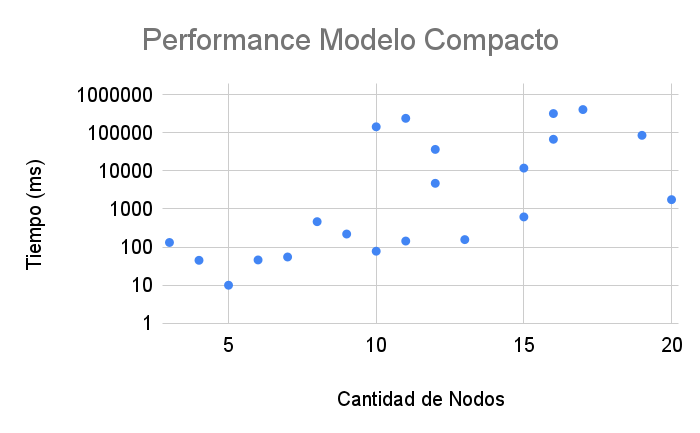
\includegraphics[width=\textwidth]{img/Performance Modelo Compacto.png}
         \caption{Modelo Compacto}
     \end{subfigure}
     \hfill
     \begin{subfigure}[b]{0.45\textwidth}
         \centering
         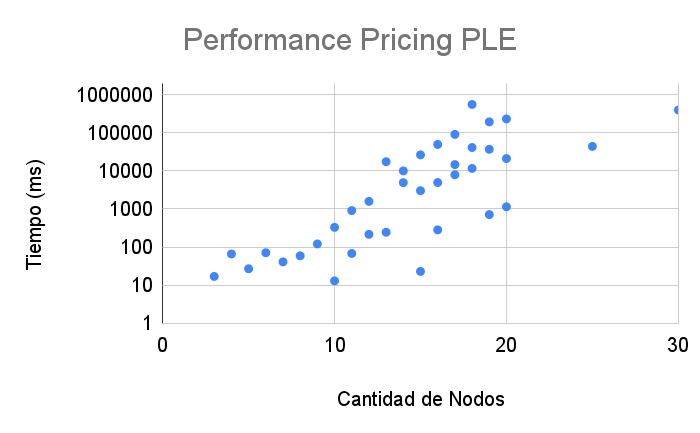
\includegraphics[width=\textwidth]{img/Performance Pricing PLE.png}
         \caption{Pricing con PLE}
     \end{subfigure}

     \begin{subfigure}[b]{0.45\textwidth}
         \centering
         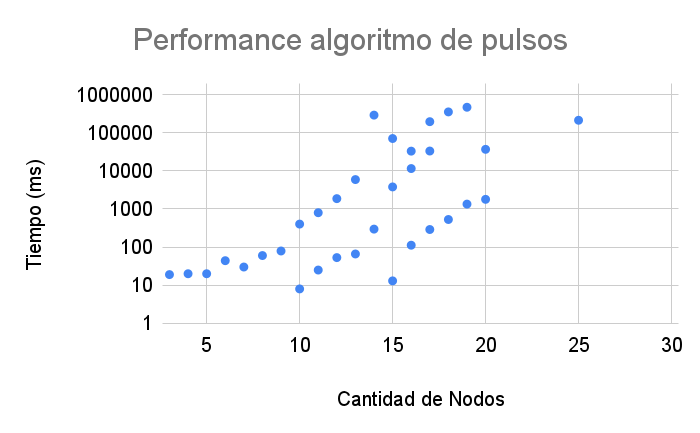
\includegraphics[width=\textwidth]{img/Performance algoritmo de pulsos.png}
         \caption{Pricing por pulsos}
     \end{subfigure}
     \hfill
     \begin{subfigure}[b]{0.45\textwidth}
         \centering
         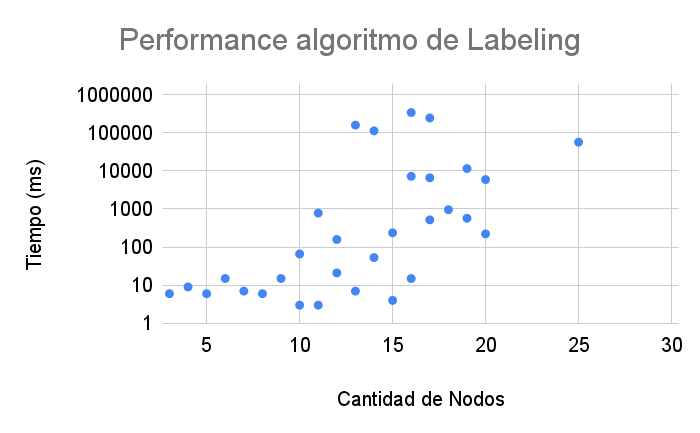
\includegraphics[width=\textwidth]{img/Performance algoritmo de Labeling.png}
         \caption{Label Setting}
     \end{subfigure}

        \caption{Tiempo vs. Cantidad de Nodos}
        \label{fig:performance-nodes}
\end{figure}

El próximo gráfico es muy similar pero ahora muestra la relación del tiempo con respecto a la cantidad de clientes en vez de nodos. La tendencia es muy parecida al caso anterior. Se podría discutir que en este caso el cúmulo de puntos se ajusta mejor a la linea que define la tendencia, que no sabemos calcular pero que demuestra el hecho de que la cantidad de clientes es una métrica un poco más fiel para predecir el tiempo total de ejecución. En la práctica sacar una conclusión de este estilo es demasiado fuerte y se sugiere fuertemente utilizar una combinación de ambos criterios.


\begin{figure}[H]
     \centering
     \begin{subfigure}[b]{0.45\textwidth}
         \centering
         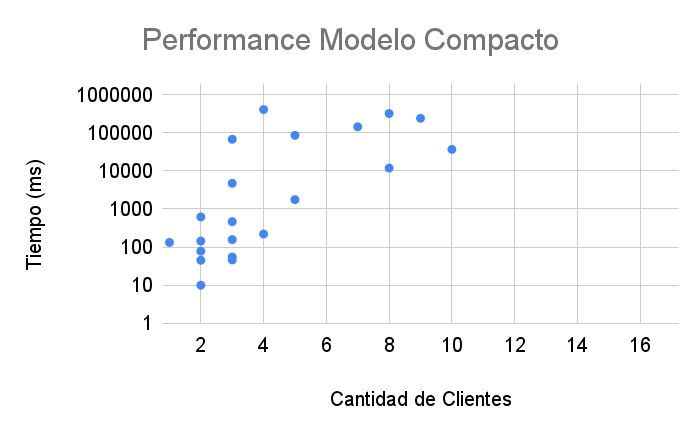
\includegraphics[width=\textwidth]{img/Performance Modelo Compacto (1).png}
         \caption{Modelo Compacto}
     \end{subfigure}
     \hfill
     \begin{subfigure}[b]{0.45\textwidth}
         \centering
         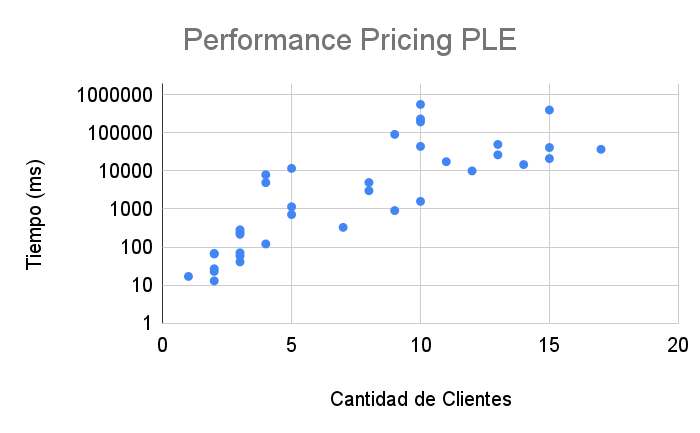
\includegraphics[width=\textwidth]{img/Performance Pricing PLE (1).png}
         \caption{Pricing con PLE}
     \end{subfigure}

     \begin{subfigure}[b]{0.45\textwidth}
         \centering
         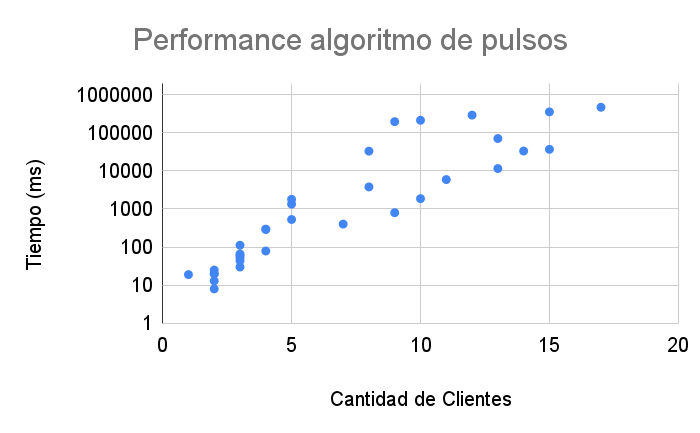
\includegraphics[width=\textwidth]{img/Performance algoritmo de pulsos (1).png}
         \caption{Pricing por pulsos}
     \end{subfigure}
     \hfill
     \begin{subfigure}[b]{0.45\textwidth}
         \centering
         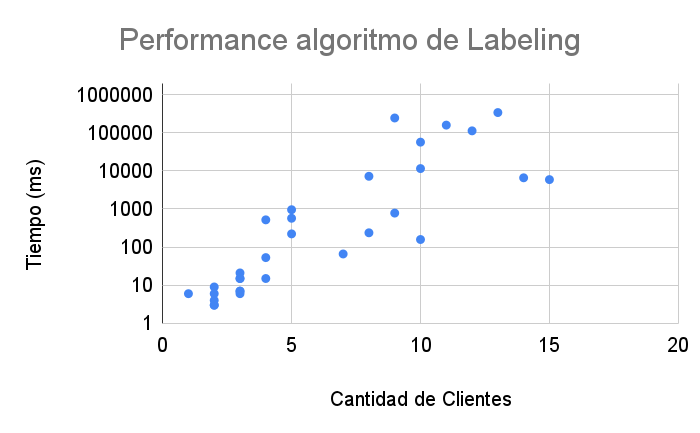
\includegraphics[width=\textwidth]{img/Performance algoritmo de Labeling (1).png}
         \caption{Label Setting}
     \end{subfigure}

        \caption{Tiempo vs. Cantidad de Clientes}
        \label{fig:performance-customers}
\end{figure}

\section{Heurísticas}

Un algoritmo de generación de columnas sin estar acompañado de Branch \& Price es una heurística en sí misma. Sin embargo, en esta sección nos referimos exclusivamente a heurísticas para resolver la relajación lineal, en particular que nos proveen una solución aproximada. 

El mecanismo que vamos a utilizar para realizar los experimentos va a ser en todos los casos el mismo: primero se corren en paralelo los algoritmos con y sin la heurística que se va a testear. Una métrica interesante sería la diferencia entre las soluciones de ambas variantes. Sin embargo, es de esperar que algunas instancias grandes solamente puedan ser corridas con el algoritmo aproximado, y por lo tanto para establecer una métrica de calidad de solución nos vamos a tener que conformar con la que veníamos utilizando hasta el momento, es decir, el gap contra el óptimo de la relajación lineal. Cabe aclarar que esta cota ahora tiene menos garantías, porque la relajación lineal también se resolvió de manera aproximada, por lo tanto este valor no es una cota inferior del óptimo real y tampoco vale que si la brecha es nula entonces el algoritmo dio la solución exacta. Con esto como motivación, existen dos métricas de calidad de solución: una que mide el gap entre la solución exacta y la aproximada (es decir, la solución encontrada con y sin la heurística en cuestión) y otra para cuando no tiene una solución exacta, que mide la brecha entre la solución del Problema Maestro con y sin restricciones de integralidad (pero en ambos casos utilizando la heurística). Para no incurrir en redundancias, las columnas restantes son análogas a los experimentos anteriores.

\subsection{Heurísticas de Label Setting}
\label{section:experiments-label-setting-heur}

La heurística que se propone en la Sección \ref{subsubsection:segment-tree-heuristic}, donde se relajan las condiciones de dominancia y eso permite hacer mucho más eficiente la estructura de datos que almacena las etiquetas y verifica si una domina a otra. Además esta estructura provee una cota superior a la cantidad de etiquetas almacenada que es mucho más ajustada que en el caso general. Otra ventaja que podemos sacar de esto es que el proceso que implica chequear si una etiqueta es dominada es más eficiente porque el \texttt{Segment Tree} tiene una complejidad logarítmica para operaciones de consulta. 

Todas estas características juntas producen tiempos mucho mejores, como se pueden explicar en la siguiente tabla. La mejora que produce esta heurística es sorprendente y sin dudas uno de los hallazgos importantes de esta tesis. El rendimiento mejora en casi la totalidad de las instancias.

En este experimento naturalmente estamos comparando el algoritmo con las heurísticas que queremos analizar contra el algoritmo estándar de labeling que resuelve la relajación lineal a exactitud. Para cada uno de estos dos algoritmos, se registran el tiempo de ejecución y la cantidad de iteraciones de generación de columnas. La columna $\Delta Fobj$ hace referencia a la diferencia relativa entre los valores de la función objetivo en ambos algoritmos. Por otro lado, muchas veces no es posible calcular esta diferencia porque el algoritmo exacto no completó la ejecución y de esta manera no hay valor contra el cual comparar. Para esto agregamos una segunda columna que intenta dar una métrica de error, midiendo el gap con respecto a la cota inferior que veníamos utilizando hasta ahora, que es el valor objetivo en la relajación lineal.

\begin{landscape}


\begin{longtblr}[
  caption = {Comparación entre labeling exacto y aproximado},
]{
  colspec = {|lrrrrrrrrr|},
  rowhead = 1,
  hlines,
  row{even} = {gray9},
} 

Instancia    & \textbar{}N\textbar{} & \textbar{}S\textbar{} & \textbar{}K\textbar{} & T s/Heur. (ms)& \#Iter s/Heur.& T c/Heur. (ms)& \#Iter c/Heur.& $\Delta Fobj$& Gap
\\ 
\hline
n3\_s1\_k1   & 3                     & 1                     & 1                     & 238       & 1              & 4         & 1              & 0.00\%                   & 0.00\%      \\
n4\_s2\_k1   & 4                     & 2                     & 1                     & 18        & 4              & 22        & 4              & 0.00\%                   & 0.00\%      \\
n5\_s2\_k1   & 5                     & 2                     & 1                     & 25        & 4              & 25        & 4              & 0.00\%                   & 0.00\%      \\
n6\_s3\_k2   & 6                     & 3                     & 2                     & 55        & 4              & 50        & 4              & 0.00\%                   & 0.00\%      \\
n7\_s3\_k2   & 7                     & 3                     & 2                     & 29        & 3              & 12        & 3              & 0.00\%                   & 0.00\%      \\
n8\_s3\_k2   & 8                     & 3                     & 2                     & 47        & 4              & 28        & 4              & 0.00\%                   & 0.00\%      \\
n9\_s4\_k2   & 9                     & 4                     & 2                     & 44        & 4              & 27        & 4              & 0.00\%                   & 0.00\%      \\
n10\_s7\_k3  & 10                    & 7                     & 3                     & 161       & 6              & 46        & 6              & 0.00\%                   & 0.00\%      \\
n10\_s2\_k2  & 10                    & 2                     & 2                     & 9         & 1              & 3         & 1              & 0.00\%                   & 0.00\%      \\
n11\_s9\_k3  & 11                    & 9                     & 3                     & 851       & 11             & 47        & 9              & 6.82\%                & 0.00\%      \\
n11\_s2\_k2  & 11                    & 2                     & 2                     & 5         & 3              & 4         & 3              & 0.00\%                   & 0.00\%      \\
n12\_s10\_k3 & 12                    & 10                    & 3                     & 178       & 11             & 34        & 11             & 0.00\%                   & 0.00\%      \\
n12\_s3\_k2  & 12                    & 3                     & 2                     & 14        & 3              & 10        & 3              & 0.00\%                   & 0.00\%      \\
n13\_s3\_k2  & 13                    & 3                     & 2                     & 9         & 4              & 4         & 4              & 0.00\%                   & 0.00\%      \\
n13\_s11\_k3 & 13                    & 11                    & 3                     & 168685    & 14             & 105       & 14             & 0.00\%                   & 12.92\%  \\
n14\_s12\_k3 & 14                    & 12                    & 3                     & 110422    & 17             & 79        & 14             & 0.00\%                   & 4.35\%   \\
n14\_s4\_k2  & 14                    & 4                     & 2                     & 49        & 6              & 8         & 6              & 0.00\%                   & 0.00\%      \\
n15\_s2\_k2  & 15                    & 2                     & 2                     & 4         & 1              & 1         & 1              & 0.00\%                   & 0.00\%      \\
n15\_s13\_k4 & 15                    & 13                    & 4                     & TLE       & 19             & 117       & 17             & ---                   & 0.71\%   \\
n15\_s8\_k2  & 15                    & 8                     & 2                     & 269       & 12             & 37        & 12             & 0.00\%                   & 0.00\%      \\
n16\_s13\_k4 & 16                    & 13                    & 4                     & 345975    & 17             & 116       & 16             & 0.00\%                   & 0.51\%   \\
n16\_s8\_k2  & 16                    & 8                     & 2                     & 7034      & 14             & 33        & 11             & 0.00\%                   & 1.79\%   \\
n16\_s3\_k2  & 16                    & 3                     & 2                     & 16        & 4              & 5         & 4              & 0.00\%                   & 0.00\%      \\
n17\_s14\_k4 & 17                    & 14                    & 4                     & 6366      & 19             & 91        & 18             & 0.00\%                   & 0.84\%   \\
n17\_s4\_k2  & 17                    & 4                     & 2                     & 519       & 6              & 12        & 6              & 0.00\%                   & 0.00\%      \\
n17\_s9\_k2  & 17                    & 9                     & 2                     & 250728    & 18             & 113       & 18             & 0.00\%                   & 0.00\%      \\
n18\_s5\_k2  & 18                    & 5                     & 2                     & 945       & 5              & 61        & 5              & 0.00\%                   & 0.00\%      \\
n18\_s10\_k2 & 18                    & 10                    & 2                     & TLE       & 19             & 167       & 14             & ---                   & 0.00\%      \\
n18\_s15\_k4 & 18                    & 15                    & 4                     & TLE       & 18             & 158       & 18             & ---                   & 9.66\%   \\
n19\_s5\_k2  & 19                    & 5                     & 2                     & 545       & 8              & 20        & 7              & 0.00\%                   & 0.00\%      \\
n19\_s17\_k4 & 19                    & 17                    & 4                     & TLE       & 22             & 291       & 22             & ---                   & 3.26\%   \\
n19\_s10\_k2 & 19                    & 10                    & 2                     & 11219     & 17             & 78        & 15             & 0.00\%                   & 0.00\%      \\
n20\_s15\_k5 & 20                    & 15                    & 5                     & 5745      & 17             & 151       & 17             & 0.00\%                   & 4.17\%   \\
n20\_s10\_k2 & 20                    & 10                    & 2                     & TLE       & 17             & 225       & 17             & ---                   & 2.20\%   \\
n20\_s5\_k2  & 20                    & 5                     & 2                     & 213       & 7              & 13        & 7              & 0.00\%                   & 0.00\%      \\
n25\_s15\_k3 & 25                    & 15                    & 3                     & TLE       & 20             & 1094      & 20             & ---                   & 5.01\%   \\
n25\_s10\_k2 & 25                    & 10                    & 2                     & 55530     & 28             & 224       & 27             & 0.00\%                   & 0.00\%      \\
n25\_s20\_k5 & 25                    & 20                    & 5                     & TLE       & 24             & 7866      & 24             & ---                   & 10.59\%  \\
n30\_s20\_k3 & 30                    & 20                    & 3                     & TLE       & 34             & 3485      & 34             & ---                   & 3.82\%   \\
n30\_s15\_k2 & 30                    & 15                    & 2                     & TLE       & 27             & 982       & 27             & ---                   & 4.81\%   \\
n30\_s25\_k5 & 30                    & 25                    & 5                     & TLE       & 35             & 6467      & 35             & ---                   & 1.63\%   \\
n35\_s20\_k3 & 35                    & 20                    & 3                     & TLE       & 19             & 11450     & 32             & ---                   & 6.22\%   \\
n35\_s15\_k2 & 35                    & 15                    & 2                     & TLE       & 23             & 6244      & 29             & ---                   & 0.00\%      \\
n35\_s25\_k5 & 35                    & 25                    & 5                     & TLE       & 34             & 4612      & 34             & ---                   & 1.40\%   \\
n40\_s20\_k3 & 40                    & 20                    & 3                     & TLE       & 10             & 139188    & 60             & ---                   & 2.67\%   \\
n40\_s15\_k2 & 40                    & 15                    & 2                     & TLE       & 15             & 9243      & 34             & ---                   & 1.30\%   \\
n40\_s30\_k5 & 40                    & 30                    & 5                     & TLE       & 11             & 31271     & 40             & ---                   & 6.50\%   \\
n45\_s20\_k3 & 45                    & 20                    & 3                     & TLE       & 11             & 18615     & 30             & ---                   & 4.26\%   \\
n45\_s40\_k5 & 45                    & 40                    & 5                     & TLE       & 9              & 142394    & 64             & ---                   & 6.23\%   \\
n45\_s15\_k2 & 45                    & 15                    & 2                     & TLE       & 12             & 16576     & 34             & ---                   & 0.00\%      \\
n50\_s45\_k5 & 50                    & 45                    & 5                     & TLE       & 10             & 169553    & 83             & ---                   & 3.01\%   \\
n50\_s10\_k2 & 50                    & 10                    & 2                     & TLE       & 15             & 987       & 15             & ---                   & 0.00\%      \\
n50\_s20\_k3 & 50                    & 20                    & 3                     & TLE       & 11             & 33167     & 36             & ---                   & 2.75\%   \\
n55\_s20\_k3 & 55                    & 20                    & 3                     & TLE       & 8              & 28380     & 31             & ---                   & 3.97\%   \\
n55\_s10\_k2 & 55                    & 10                    & 2                     & TLE       & 17             & 4428      & 17             & ---                   & 5.09\%   \\
n55\_s45\_k5 & 55                    & 45                    & 5                     & TLE       & 9              & 422897    & 92             & ---                   & 2.36\%   \\
n60\_s10\_k2 & 60                    & 10                    & 2                     & TLE       & 8              & 8716      & 15             & ---                   & 7.90\%   \\
n60\_s20\_k3 & 60                    & 20                    & 3                     & TLE       & 7              & 172342    & 52             & ---                   & 1.54\%   \\
n60\_s50\_k5 & 60                    & 50                    & 5                     & TLE       & 4              & TLE       & 71             & ---                   & ---      \\
n65\_s10\_k2 & 65                    & 10                    & 2                     & TLE       & 15             & 5259      & 20             & ---                   & 0.00\%      \\
n65\_s20\_k3 & 65                    & 20                    & 3                     & TLE       & 9              & 95444     & 37             & ---                   & 0.00\%      \\
n65\_s55\_k5 & 65                    & 55                    & 5                     & TLE       & 6              & TLE       & 13             & ---                   & ---      \\
n70\_s10\_k2 & 70                    & 10                    & 2                     & TLE       & 5              & 46446     & 25             & ---                   & 5.56\%   \\
\hline
\end{longtblr}
\end{landscape}

Es claro que este algoritmo es mucho más rápido que los que resuelven el pricing con exactitud, dado que pudimos procesar instancias mucho más grandes, hasta 70 nodos y 45 clientes. Es digno de discusión si vale la pena sacrificar la garantía de exactitud para tener un gran incremento en rendimiento, incluso viendo que la pérdida de calidad de la solución no es muy grande en los casos que se pudo computar. En particular, solamente 2 instancias tienen un gap contra la cota inferior que es superior al $10.00\%$, aunque recordemos que al tratarse de una heurística perdemos la garantía de que la solución de la relajación lineal sea una cota inferior del óptimo real.

Es alentador ver que 30 filas cumplen que $\Delta Fobj = 0.00\%$; eso significa que la solución aproximada coincide con la exacta, por lo tanto, decimos que se ``adivinó'' el verdadero valor del óptimo de la función objetivo. Lamentablemente no podemos extrapolar este resultado a instancias relativamente grandes porque el algoritmo exacto no termina la ejecución y por consiguiente tampoco podemos calcular la diferencia. Asimismo hay 31 de 63 instancias cuyo gap es 0, y también podemos extraer que 61 de ellas terminaron la ejecución.   


\subsection{2-Step Column Generation}
\label{section:2-step-cg-testing}

Las técnicas que se describen en \ref{section:2-step-cg} sirven para reducir marginalmente la cantidad de iteraciones de generación de columnas y en el caso de combinarse con un algoritmo aproximado, apunta a mejorar el valor de la función objetivo porque agrega a la base posibilidades que el pricing estándar desconoce. Con esto en mente, tiene sentido que la comparación de este experimento sea en base a un pricing aproximado, porque el efecto se aprecia mejor cuando hay muchas iteraciones. En esta subsección aplicamos la heurística de 2-Step Column Generation utilizando como pricing el algoritmo de Label Setting aproximado, es decir, ambas heurísticas al mismo tiempo. Es de esperar que en instancias chicas el overhead de aplicar este procedimiento dé tiempos más elevados, por lo tanto vale la pena solamente considerarlo a partir de cierto número de clientes. 

Cuando se mide el gap exacto, es decir, la diferencia porcentual entre la solución con y sin heurística respectivamente, el valor puede ser positivo o negativo, ya que se mide el incremento porcentual del valor con heurística con respecto al que no la aplica. Es decir, si el valor con heurística es menor al que no tiene heurística, este número será negativo. Como ambos entregan soluciones factibles, el que dé el menor valor estará más cerca del óptimo, y por lo tanto, en caso de que este algoritmo sea útil y 2-Step Column Generation mejore la solución, esperaríamos ver muchas columnas con valores negativos.

En la tabla que sigue medimos el tiempo en milisegundos tomado por los algoritmos con y sin esta mejora (en la columna ``T''), así como también la cantidad de iteraciones. Al igual que en el experimento anterior, se indican la diferencia entre los valores de la función objetivo entre dichas alternativas y el gap con respecto a la relajación lineal. 


\begin{landscape}
\begin{longtblr}[
  caption = {Comparación de Generación de Columnas con y sin 2-Step Column Generation},
]{
  colspec = {|lrrrrrrrrr|},
  rowhead = 1,
  hlines,
  row{even} = {gray9},
} 

Instancia    & \textbar{}N\textbar{} & \textbar{}S\textbar{} & \textbar{}K\textbar{} & T s/2GC (ms)& \#Iter s/2GC & T c/2GC (ms)& \#Iter c/2GC& $\Delta Fobj$& Gap
\\ 
\hline
n3\_s1\_k1   & 3                     & 1                     & 1                     & 130                 & 1                 & 3                   & 1                 & 0.00\%        & 0.00\%         \\
n4\_s2\_k1   & 4                     & 2                     & 1                     & 12                  & 4                 & 13                  & 4                 & 0.00\%        & 0.00\%         \\
n5\_s2\_k1   & 5                     & 2                     & 1                     & 9                   & 4                 & 10                  & 4                 & 0.00\%        & 0.00\%         \\
n6\_s3\_k2   & 6                     & 3                     & 2                     & 27                  & 4                 & 29                  & 3                 & 0.00\%        & 0.00\%         \\
n7\_s3\_k2   & 7                     & 3                     & 2                     & 14                  & 3                 & 10                  & 3                 & 0.00\%        & 0.00\%         \\
n8\_s3\_k2   & 8                     & 3                     & 2                     & 13                  & 4                 & 9                   & 4                 & 0.00\%        & 0.00\%         \\
n9\_s4\_k2   & 9                     & 4                     & 2                     & 17                  & 4                 & 14                  & 4                 & 0.00\%        & 0.00\%         \\
n10\_s7\_k3  & 10                    & 7                     & 3                     & 34                  & 6                 & 63                  & 7                 & 0.00\%        & 0.00\%         \\
n10\_s2\_k2  & 10                    & 2                     & 2                     & 3                   & 1                 & 2                   & 1                 & 0.00\%        & 0.00\%         \\
n11\_s9\_k3  & 11                    & 9                     & 3                     & 127                 & 9                 & 102                 & 11                & -6.38\%    & 0.00\%         \\
n11\_s2\_k2  & 11                    & 2                     & 2                     & 6                   & 3                 & 7                   & 3                 & 0.00\%        & 0.00\%         \\
n12\_s10\_k3 & 12                    & 10                    & 3                     & 76                  & 11                & 111                 & 11                & 0.00\%        & 0.00\%         \\
n12\_s3\_k2  & 12                    & 3                     & 2                     & 55                  & 3                 & 23                  & 3                 & 0.00\%        & 0.00\%         \\
n13\_s3\_k2  & 13                    & 3                     & 2                     & 8                   & 4                 & 6                   & 4                 & 0.00\%        & 0.00\%         \\
n13\_s11\_k3 & 13                    & 11                    & 3                     & 228                 & 14                & 97                  & 12                & 1.49\%     & 14.61\%     \\
n14\_s12\_k3 & 14                    & 12                    & 3                     & 88                  & 14                & 178                 & 21                & -5\%       & 7.55\%      \\
n14\_s4\_k2  & 14                    & 4                     & 2                     & 8                   & 6                 & 9                   & 6                 & 0.00\%        & 0.00\%         \\
n15\_s2\_k2  & 15                    & 2                     & 2                     & 2                   & 1                 & 2                   & 1                 & 0.00\%        & 0.00\%         \\
n15\_s13\_k4 & 15                    & 13                    & 4                     & 122                 & 17                & 138                 & 19                & 2.82\%     & 4.29\%      \\
n15\_s8\_k2  & 15                    & 8                     & 2                     & 33                  & 12                & 37                  & 11                & 0.00\%        & 0.00\%         \\
n16\_s13\_k4 & 16                    & 13                    & 4                     & 126                 & 16                & 125                 & 14                & 0.00\%        & 0.51\%      \\
n16\_s8\_k2  & 16                    & 8                     & 2                     & 38                  & 11                & 46                  & 10                & 0.00\%        & 1.79\%      \\
n16\_s3\_k2  & 16                    & 3                     & 2                     & 5                   & 4                 & 5                   & 4                 & 0.00\%        & 0.00\%         \\
n17\_s14\_k4 & 17                    & 14                    & 4                     & 84                  & 18                & 72                  & 15                & 0.00\%        & 0.84\%      \\
n17\_s4\_k2  & 17                    & 4                     & 2                     & 11                  & 6                 & 18                  & 6                 & 0.00\%        & 0.00\%         \\
n17\_s9\_k2  & 17                    & 9                     & 2                     & 109                 & 18                & 136                 & 15                & 0.00\%        & 0.00\%         \\
n18\_s5\_k2  & 18                    & 5                     & 2                     & 69                  & 5                 & 62                  & 9                 & 0.00\%        & 0.00\%         \\
n18\_s10\_k2 & 18                    & 10                    & 2                     & 166                 & 14                & 225                 & 16                & 3.45\%     & 0.00\%         \\
n18\_s15\_k4 & 18                    & 15                    & 4                     & 162                 & 18                & 214                 & 15                & -2.38\%    & 8.75\%      \\
n19\_s5\_k2  & 19                    & 5                     & 2                     & 21                  & 7                 & 12                  & 4                 & 0.00\%        & 0.90\%      \\
n19\_s17\_k4 & 19                    & 17                    & 4                     & 295                 & 22                & 220                 & 17                & 0.00\%        & 3.26\%      \\
n19\_s10\_k2 & 19                    & 10                    & 2                     & 81                  & 15                & 73                  & 15                & 0.00\%        & 0.00\%         \\
n20\_s15\_k5 & 20                    & 15                    & 5                     & 119                 & 17                & 84                  & 10                & 0.00\%        & 4.17\%      \\
n20\_s10\_k2 & 20                    & 10                    & 2                     & 214                 & 17                & 157                 & 15                & -7.06\%    & 0.00\%         \\
n20\_s5\_k2  & 20                    & 5                     & 2                     & 16                  & 7                 & 17                  & 7                 & 0.00\%        & 0.00\%         \\
n25\_s15\_k3 & 25                    & 15                    & 3                     & 1119                & 20                & 984                 & 20                & 2.29\%     & 7.20\%      \\
n25\_s10\_k2 & 25                    & 10                    & 2                     & 205                 & 27                & 181                 & 17                & 0.00\%        & 0.00\%         \\
n25\_s20\_k5 & 25                    & 20                    & 5                     & 7637                & 24                & 6437                & 24                & 0.00\%        & 10.50\%     \\
n30\_s20\_k3 & 30                    & 20                    & 3                     & 3377                & 34                & 4335                & 33                & -4.41\%    & 0.29\%      \\
n30\_s15\_k2 & 30                    & 15                    & 2                     & 1009                & 27                & 675                 & 25                & 1.02\%     & 5.10\%      \\
n30\_s25\_k5 & 30                    & 25                    & 5                     & 5937                & 35                & 4261                & 22                & 1.35\%     & 2.74\%      \\
n35\_s20\_k3 & 35                    & 20                    & 3                     & 10633               & 32                & 17403               & 28                & 0.00\%        & 6.02\%      \\
n35\_s15\_k2 & 35                    & 15                    & 2                     & 5955                & 29                & 9397                & 28                & -2.94\%    & 0.00\%         \\
n35\_s25\_k5 & 35                    & 25                    & 5                     & 4493                & 34                & 2894                & 27                & 0.55\%     & 1.68\%      \\
n40\_s20\_k3 & 40                    & 20                    & 3                     & 132799              & 60                & 58279               & 37                & 0.58\%     & 2.65\%      \\
n40\_s15\_k2 & 40                    & 15                    & 2                     & 9138                & 34                & 9148                & 36                & -5.15\%    & 0.00\%         \\
n40\_s30\_k5 & 40                    & 30                    & 5                     & 29496               & 40                & 33791               & 32                & -2.51\%    & 3.91\%      \\
n45\_s20\_k3 & 45                    & 20                    & 3                     & 17452               & 30                & 15749               & 29                & -4.40\%    & 0.00\%         \\
n45\_s40\_k5 & 45                    & 40                    & 5                     & 134447              & 64                & 151769              & 57                & -2.06\%    & 4.27\%      \\
n45\_s15\_k2 & 45                    & 15                    & 2                     & 16168               & 34                & 10852               & 26                & 0.00\%        & 0.00\%         \\
n50\_s45\_k5 & 50                    & 45                    & 5                     & 160539              & 83                & 87726               & 62                & 0.00\%        & 3.60\%      \\
n50\_s10\_k2 & 50                    & 10                    & 2                     & 963                 & 15                & 951                 & 14                & 0.00\%        & 1.20\%      \\
n50\_s20\_k3 & 50                    & 20                    & 3                     & 31134               & 36                & 13042               & 34                & -0.70\%    & 1.97\%      \\
n55\_s20\_k3 & 55                    & 20                    & 3                     & 27149               & 31                & 26015               & 26                & -0.46\%    & 3.90\%      \\
n55\_s10\_k2 & 55                    & 10                    & 2                     & 4277                & 17                & 4983                & 16                & 1.15\%     & 5.60\%      \\
n55\_s45\_k5 & 55                    & 45                    & 5                     & 399056              & 92                & 487636              & 76                & -0.42\%    & 4.94\%      \\
n60\_s10\_k2 & 60                    & 10                    & 2                     & 8588                & 15                & 10083               & 20                & 0.00\%        & 8.28\%      \\
n60\_s20\_k3 & 60                    & 20                    & 3                     & 165413              & 52                & 121311              & 29                & 6.70\%     & 4.77\%      \\
n60\_s50\_k5 & 60                    & 50                    & 5                     & TLE                 & 74                & TLE                 & 58                & ---        & ---         \\
n65\_s10\_k2 & 65                    & 10                    & 2                     & 5312                & 20                & 3883                & 13                & -29.66\%   & 0.00\%         \\
n65\_s20\_k3 & 65                    & 20                    & 3                     & 93359               & 37                & 199589              & 27                & 0.00\%        & 0.41\%      \\
n65\_s55\_k5 & 65                    & 55                    & 5                     & TLE                 & 13                & TLE                 & 10                & ---        & ---         \\
n70\_s10\_k2 & 70                    & 10                    & 2                     & 47371               & 25                & 33866               & 19                & 0.00\%        & 5.44\%      \\
\hline
\end{longtblr}
\end{landscape}


Dado que estamos corriendo la heurística de 2-Step Column Generation combinada con el algoritmo de labeling aproximado, que es lo mismo que testeamos en el experimento de la subsección anterior (Subsección \ref{section:experiments-label-setting-heur}) tiene sentido comparar los resultados de esta subsección con los de la anterior. 

Si bien el rendimiento en general no se ve sustancialmente beneficiado por esta nueva propuesta, vale la pena considerar una heurística como ésta porque cumple su objetivo fundamental: la cantidad de iteraciones se ve reducida consistentemente. De las 63 instancias que se corrieron en ambos experimentos, en 35 fue más eficiente la implementación con 2-Step Column Generation, en 26 la heurística que sólo usa el labeling aproximado venció, y en 2 ambas resultaron en TLE. Sin embargo, en 53 ocasiones la cantidad de iteraciones disminuyó.

La calidad de la solución también mejora en un porcentaje sensible con respecto al experimento anterior, ya que en 14 instancias obtuvimos un valor en la función objetivo mejor que solamente con el labeling, contra 10 donde esto fue al revés (el resto dan iguales o bien no se puede determinar).


\subsection{Terminación temprana}

Un último experimento nos permite verificar el impacto de la heurística de terminación temprana. Como explicamos en la Sección \ref{section:finish-early}, estamos obligados a que el problema de pricing se resuelva a optimalidad, por que sino no es válido el teorema en el que se basa la condición de terminación. Resulta apropiado para esta prueba comparar ambos algoritmos (con y sin terminación temprana) utilizando como solver del problema de pricing el algoritmo por pulsos exacto. Respectivamente utilizamos las siglas ``c/TT'' y ``s/TT'' en las columnas de la siguiente tabla para indicar que el algoritmo se corrió con y sin terminación temprana. 

En este caso, el valor que se eligió de para limitar el error es de $5\%$, a partir del cual se habilita la terminación temprana. Es discutible si este número es alto o no para instancias prácticas, pero a fines puramente teóricos queríamos tener un valor que evidencie sus propiedades. En este experimento utilizamos el pricing exacto con algoritmo de labeling. Por lo tanto tendría sentido comparar los resultados con los de la tabla en la Subsección \ref{section:experiment-labeling}.

Realmente solo tiene sentido comparar las entradas donde la cantidad de iteraciones se ve reducida, ya que en los otros casos la diferencia de tiempo se explica meramente en base a pequeñas diferencias usuales del entorno, y no por cuestiones inherentes al algoritmo. La fortaleza de esta heurística es que la degradación de la solución ya está acotada de antemano, entonces el error está limitado, pero la ganancia de tiempo no lo está. Idealmente, en instancias más grandes donde haya muchas iteraciones, se podría ver el verdadero efecto.

Observamos que de las 37 instancias, en 28 el valor de la función objetivo fue el mismo que sin aplicar la heurística, y por lo tanto no se degradó la solución. Además, las mismas 4 instancias que resultaron en TLE con la heurística también lo hicieron sin ésta. La motivación principal de este experimento es probar que esta heurística es eficiente para reducir los tiempos de ejecución y en particular para reducir la cantidad de iteraciones. En 14 casos de los 37 logramos reducir este número. Como dijimos, comparar la columna de tiempos no tiene sentido porque ambos corren el mismo algoritmo, y la única diferencia es que uno corta antes. 

En cuanto a la calidad de la solución, solamente hay un caso inaceptable donde solución quedó muy lejos de la exacta.  

\begin{landscape}
\begin{longtblr}[
  caption = {Comparación de Generación de Columnas con y sin terminación temprana},
]{
  colspec = {|lrrrrrrrrr|},
  rowhead = 1,
  hlines,
  row{even} = {gray9},
} 

Instancia    & \textbar{}N\textbar{} & \textbar{}S\textbar{} & \textbar{}K\textbar{} & T s/TT (ms)& \#Iter s/TT& T c/TT (ms)& \#Iter c/TT& $\Delta Fobj$& Gap
\\ 
\hline
n3\_s1\_k1   & 3                     & 1                     & 1                     & 153                 & 1                 & 5                   & 1                 & 0.00\%        & 0.00\%         \\
n4\_s2\_k1   & 4                     & 2                     & 1                     & 53                  & 4                 & 34                  & 4                 & 0.00\%        & 0.00\%         \\
n5\_s2\_k1   & 5                     & 2                     & 1                     & 31                  & 4                 & 24                  & 4                 & 0.00\%        & 0.00\%         \\
n6\_s3\_k2   & 6                     & 3                     & 2                     & 92                  & 4                 & 94                  & 4                 & 0.00\%        & 33.33\%     \\
n7\_s3\_k2   & 7                     & 3                     & 2                     & 94                  & 3                 & 68                  & 3                 & 0.00\%        & 0.00\%         \\
n8\_s3\_k2   & 8                     & 3                     & 2                     & 130                 & 4                 & 52                  & 4                 & 0.00\%        & 0.00\%         \\
n9\_s4\_k2   & 9                     & 4                     & 2                     & 49                  & 4                 & 48                  & 4                 & 0.00\%        & 0.00\%         \\
n10\_s7\_k3  & 10                    & 7                     & 3                     & 287                 & 10                & 261                 & 10                & 0.00\%        & 0.00\%         \\
n10\_s2\_k2  & 10                    & 2                     & 2                     & 8                   & 1                 & 8                   & 1                 & 0.00\%        & 0.00\%         \\
n11\_s9\_k3  & 11                    & 9                     & 3                     & 825                 & 13                & 820                 & 13                & 0.00\%        & 0.00\%         \\
n11\_s2\_k2  & 11                    & 2                     & 2                     & 30                  & 3                 & 26                  & 3                 & 0.00\%        & 0.00\%         \\
n12\_s10\_k3 & 12                    & 10                    & 3                     & 1953                & 17                & 1936                & 17                & 0.00\%        & 0.00\%         \\
n12\_s3\_k2  & 12                    & 3                     & 2                     & 45                  & 4                 & 46                  & 4                 & 0.00\%        & 0.00\%         \\
n13\_s3\_k2  & 13                    & 3                     & 2                     & 65                  & 4                 & 62                  & 4                 & 0.00\%        & 0.00\%         \\
n13\_s11\_k3 & 13                    & 11                    & 3                     & 5985                & 20                & 6230                & 19                & 0.00\%        & 14.61\%     \\
n14\_s12\_k3 & 14                    & 12                    & 3                     & 299443              & 26                & 296396              & 26                & 0.00\%        & 4.35\%      \\
n14\_s4\_k2  & 14                    & 4                     & 2                     & 296                 & 7                 & 299                 & 7                 & 0.00\%        & 0.00\%         \\
n15\_s2\_k2  & 15                    & 2                     & 2                     & 13                  & 1                 & 13                  & 1                 & 0.00\%        & 0.00\%         \\
n15\_s13\_k4 & 15                    & 13                    & 4                     & 73893               & 25                & 71344               & 24                & 5.63\%     & 7.96\%      \\
n15\_s8\_k2  & 15                    & 8                     & 2                     & 3856                & 19                & 2953                & 14                & 0.00\%        & 0.00\%         \\
n16\_s13\_k4 & 16                    & 13                    & 4                     & 12021               & 21                & 10798               & 17                & 1.02\%     & 1.28\%      \\
n16\_s8\_k2  & 16                    & 8                     & 2                     & 35648               & 17                & 34967               & 15                & 0.00\%        & 12.05\%     \\
n16\_s3\_k2  & 16                    & 3                     & 2                     & 111                 & 5                 & 111                 & 5                 & 0.00\%        & 0.00\%         \\
n17\_s14\_k4 & 17                    & 14                    & 4                     & 34787               & 21                & 34796               & 21                & 0.00\%        & 6.58\%      \\
n17\_s4\_k2  & 17                    & 4                     & 2                     & 279                 & 5                 & 283                 & 5                 & 0.00\%        & 0.00\%         \\
n17\_s9\_k2  & 17                    & 9                     & 2                     & 208433              & 22                & 203256              & 20                & 3.17\%     & 2.09\%      \\
n18\_s5\_k2  & 18                    & 5                     & 2                     & 562                 & 8                 & 554                 & 8                 & 0.00\%        & 0.00\%         \\
n18\_s10\_k2 & 18                    & 10                    & 2                     & TLE                 & 13                & TLE                 & 13                & ---        & ---         \\
n18\_s15\_k4 & 18                    & 15                    & 4                     & 350970              & 24                & 347182              & 22                & 0.00\%        & 9.91\%      \\
n19\_s5\_k2  & 19                    & 5                     & 2                     & 1310                & 10                & 1168                & 9                 & 0.00\%        & 0.60\%      \\
n19\_s17\_k4 & 19                    & 17                    & 4                     & 468685              & 33                & 466743              & 30                & 0.00\%        & 6.27\%      \\
n19\_s10\_k2 & 19                    & 10                    & 2                     & TLE                 & 10                & TLE                 & 10                & ---        & ---         \\
n20\_s15\_k5 & 20                    & 15                    & 5                     & 36828               & 20                & 37086               & 20                & 0.00\%        & 13.10\%     \\
n20\_s10\_k2 & 20                    & 10                    & 2                     & TLE                 & 9                 & TLE                 & 9                 & ---        & ---         \\
n20\_s5\_k2  & 20                    & 5                     & 2                     & 1766                & 10                & 1467                & 8                 & 25.81\%    & 23.81\%     \\
n25\_s15\_k3 & 25                    & 15                    & 3                     & TLE                 & 5                 & TLE                 & 5                 & ---        & ---         \\
n25\_s10\_k2 & 25                    & 10                    & 2                     & 200226              & 34                & 178031              & 19                & 1.54\%     & 0.00\%         \\
\hline
\end{longtblr}
\end{landscape}
 

